\documentclass{standalone}
\usepackage{tikz}
\usetikzlibrary{patterns, positioning}


\begin{document}
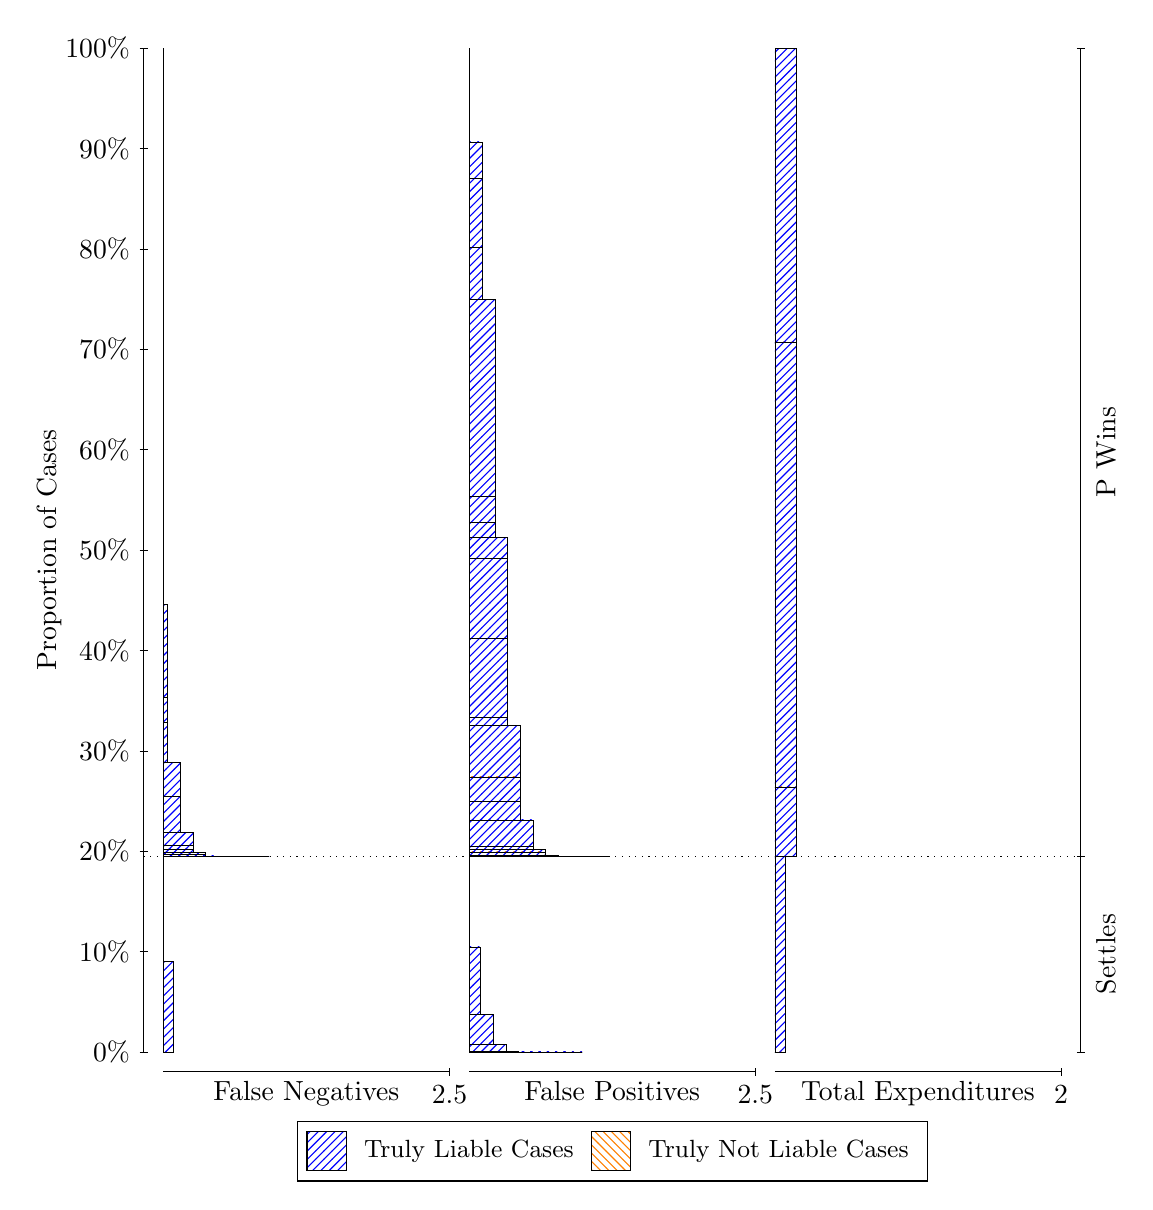
\begin{tikzpicture}
\draw[black, very thin] (1.5,1.75) -- (1.5,14.5);
\node[rotate=90, text=black, anchor=center] at (0.3, 8.125) {Proportion of Cases};
\draw[black, very thin] (1.45,1.75) -- (1.55,1.75);
\node[text=black, anchor=east] at (1.45, 1.75) {0\%};
\draw[black, very thin] (1.45,3.025) -- (1.55,3.025);
\node[text=black, anchor=east] at (1.45, 3.025) {10\%};
\draw[black, very thin] (1.45,4.3) -- (1.55,4.3);
\node[text=black, anchor=east] at (1.45, 4.3) {20\%};
\draw[black, very thin] (1.45,5.575) -- (1.55,5.575);
\node[text=black, anchor=east] at (1.45, 5.575) {30\%};
\draw[black, very thin] (1.45,6.85) -- (1.55,6.85);
\node[text=black, anchor=east] at (1.45, 6.85) {40\%};
\draw[black, very thin] (1.45,8.125) -- (1.55,8.125);
\node[text=black, anchor=east] at (1.45, 8.125) {50\%};
\draw[black, very thin] (1.45,9.4) -- (1.55,9.4);
\node[text=black, anchor=east] at (1.45, 9.4) {60\%};
\draw[black, very thin] (1.45,10.675) -- (1.55,10.675);
\node[text=black, anchor=east] at (1.45, 10.675) {70\%};
\draw[black, very thin] (1.45,11.95) -- (1.55,11.95);
\node[text=black, anchor=east] at (1.45, 11.95) {80\%};
\draw[black, very thin] (1.45,13.225) -- (1.55,13.225);
\node[text=black, anchor=east] at (1.45, 13.225) {90\%};
\draw[black, very thin] (1.45,14.5) -- (1.55,14.5);
\node[text=black, anchor=east] at (1.45, 14.5) {100\%};

\draw[black, very thin] (13.4,1.75) -- (13.4,14.5);
\draw[black, very thin] (13.35,1.75) -- (13.45,1.75);
\node[anchor=west] at (13.35, 1.75) {};
\draw[black, very thin] (13.35,4.2363) -- (13.45,4.2363);
\node[anchor=west] at (13.35, 4.2363) {};
\draw[black, very thin] (13.35,14.5) -- (13.45,14.5);
\node[anchor=west] at (13.35, 14.5) {};

\draw[black, very thin, pattern color=blue, pattern=north east lines] (1.75,1.75) rectangle (1.8772,2.9018);
\draw[black, very thin, pattern color=orange, pattern=north west lines] (1.75,2.9018) rectangle (1.75,2.9018);
\draw[black, very thin, pattern color=blue, pattern=north east lines] (1.75,2.9018) rectangle (1.75,4.2363);
\draw[black, very thin, pattern color=blue, pattern=north east lines] (1.75,4.2363) rectangle (3.0943,4.2363);
\draw[black, very thin, pattern color=blue, pattern=north east lines] (1.75,4.2363) rectangle (2.9329,4.2363);
\draw[black, very thin, pattern color=blue, pattern=north east lines] (1.75,4.2363) rectangle (2.7714,4.2363);
\draw[black, very thin, pattern color=blue, pattern=north east lines] (1.75,4.2363) rectangle (2.7714,4.2363);
\draw[black, very thin, pattern color=blue, pattern=north east lines] (1.75,4.2363) rectangle (2.6099,4.2366);
\draw[black, very thin, pattern color=blue, pattern=north east lines] (1.75,4.2366) rectangle (2.6099,4.2367);
\draw[black, very thin, pattern color=blue, pattern=north east lines] (1.75,4.2367) rectangle (2.4484,4.2369);
\draw[black, very thin, pattern color=blue, pattern=north east lines] (1.75,4.2369) rectangle (2.4484,4.2396);
\draw[black, very thin, pattern color=blue, pattern=north east lines] (1.75,4.2396) rectangle (2.4484,4.2417);
\draw[black, very thin, pattern color=blue, pattern=north east lines] (1.75,4.2417) rectangle (2.2869,4.2662);
\draw[black, very thin, pattern color=blue, pattern=north east lines] (1.75,4.2662) rectangle (2.2869,4.2872);
\draw[black, very thin, pattern color=blue, pattern=north east lines] (1.75,4.2872) rectangle (2.1254,4.33);
\draw[black, very thin, pattern color=blue, pattern=north east lines] (1.75,4.33) rectangle (2.1254,4.3782);
\draw[black, very thin, pattern color=blue, pattern=north east lines] (1.75,4.3782) rectangle (2.1254,4.5402);
\draw[black, very thin, pattern color=blue, pattern=north east lines] (1.75,4.5402) rectangle (1.964,4.9946);
\draw[black, very thin, pattern color=blue, pattern=north east lines] (1.75,4.9946) rectangle (1.964,5.4274);
\draw[black, very thin, pattern color=blue, pattern=north east lines] (1.75,5.4274) rectangle (1.8025,5.9324);
\draw[black, very thin, pattern color=blue, pattern=north east lines] (1.75,5.9324) rectangle (1.8025,6.2518);
\draw[black, very thin, pattern color=blue, pattern=north east lines] (1.75,6.2518) rectangle (1.8025,7.4335);
\draw[black, very thin, pattern color=orange, pattern=north west lines] (1.75,7.4335) rectangle (1.75,7.4335);
\draw[black, very thin, pattern color=blue, pattern=north east lines] (1.75,7.4335) rectangle (1.75,14.5);
\draw[black, very thin, pattern color=orange, pattern=north west lines] (5.6333,1.75) rectangle (7.0685,1.75);
\draw[black, very thin, pattern color=blue, pattern=north east lines] (5.6333,1.75) rectangle (7.0685,1.75);
\draw[black, very thin, pattern color=blue, pattern=north east lines] (5.6333,1.75) rectangle (6.907,1.75);
\draw[black, very thin, pattern color=blue, pattern=north east lines] (5.6333,1.75) rectangle (6.7455,1.75);
\draw[black, very thin, pattern color=blue, pattern=north east lines] (5.6333,1.75) rectangle (6.5841,1.75);
\draw[black, very thin, pattern color=blue, pattern=north east lines] (5.6333,1.75) rectangle (6.4226,1.7503);
\draw[black, very thin, pattern color=blue, pattern=north east lines] (5.6333,1.7503) rectangle (6.2611,1.7582);
\draw[black, very thin, pattern color=blue, pattern=north east lines] (5.6333,1.7582) rectangle (6.0996,1.8431);
\draw[black, very thin, pattern color=blue, pattern=north east lines] (5.6333,1.8431) rectangle (5.9381,2.231);
\draw[black, very thin, pattern color=blue, pattern=north east lines] (5.6333,2.231) rectangle (5.7766,3.0845);
\draw[black, very thin, pattern color=blue, pattern=north east lines] (5.6333,3.0845) rectangle (5.6333,4.2363);
\draw[black, very thin, pattern color=orange, pattern=north west lines] (5.6333,4.2363) rectangle (7.4137,4.2363);
\draw[black, very thin, pattern color=blue, pattern=north east lines] (5.6333,4.2363) rectangle (7.4137,4.2363);
\draw[black, very thin, pattern color=orange, pattern=north west lines] (5.6333,4.2363) rectangle (7.2522,4.2363);
\draw[black, very thin, pattern color=blue, pattern=north east lines] (5.6333,4.2363) rectangle (7.2522,4.2363);
\draw[black, very thin, pattern color=orange, pattern=north west lines] (5.6333,4.2363) rectangle (7.0907,4.2363);
\draw[black, very thin, pattern color=blue, pattern=north east lines] (5.6333,4.2363) rectangle (7.0907,4.2363);
\draw[black, very thin, pattern color=blue, pattern=north east lines] (5.6333,4.2363) rectangle (6.9292,4.2365);
\draw[black, very thin, pattern color=blue, pattern=north east lines] (5.6333,4.2365) rectangle (6.9292,4.2367);
\draw[black, very thin, pattern color=orange, pattern=north west lines] (5.6333,4.2367) rectangle (6.9292,4.2367);
\draw[black, very thin, pattern color=blue, pattern=north east lines] (5.6333,4.2367) rectangle (6.9292,4.2371);
\draw[black, very thin, pattern color=blue, pattern=north east lines] (5.6333,4.2371) rectangle (6.7677,4.2402);
\draw[black, very thin, pattern color=orange, pattern=north west lines] (5.6333,4.2402) rectangle (6.7677,4.2402);
\draw[black, very thin, pattern color=blue, pattern=north east lines] (5.6333,4.2402) rectangle (6.7677,4.2443);
\draw[black, very thin, pattern color=blue, pattern=north east lines] (5.6333,4.2443) rectangle (6.7677,4.2462);
\draw[black, very thin, pattern color=blue, pattern=north east lines] (5.6333,4.2462) rectangle (6.6063,4.2915);
\draw[black, very thin, pattern color=orange, pattern=north west lines] (5.6333,4.2915) rectangle (6.6063,4.2915);
\draw[black, very thin, pattern color=blue, pattern=north east lines] (5.6333,4.2915) rectangle (6.6063,4.3199);
\draw[black, very thin, pattern color=blue, pattern=north east lines] (5.6333,4.3199) rectangle (6.4448,4.3656);
\draw[black, very thin, pattern color=orange, pattern=north west lines] (5.6333,4.3656) rectangle (6.4448,4.3656);
\draw[black, very thin, pattern color=blue, pattern=north east lines] (5.6333,4.3656) rectangle (6.4448,4.6963);
\draw[black, very thin, pattern color=blue, pattern=north east lines] (5.6333,4.6963) rectangle (6.2833,4.9328);
\draw[black, very thin, pattern color=blue, pattern=north east lines] (5.6333,4.9328) rectangle (6.2833,5.2436);
\draw[black, very thin, pattern color=orange, pattern=north west lines] (5.6333,5.2436) rectangle (6.2833,5.2436);
\draw[black, very thin, pattern color=blue, pattern=north east lines] (5.6333,5.2436) rectangle (6.2833,5.8984);
\draw[black, very thin, pattern color=blue, pattern=north east lines] (5.6333,5.8984) rectangle (6.1218,6.004);
\draw[black, very thin, pattern color=blue, pattern=north east lines] (5.6333,6.004) rectangle (6.1218,7.0051);
\draw[black, very thin, pattern color=orange, pattern=north west lines] (5.6333,7.0051) rectangle (6.1218,7.0051);
\draw[black, very thin, pattern color=blue, pattern=north east lines] (5.6333,7.0051) rectangle (6.1218,8.0221);
\draw[black, very thin, pattern color=blue, pattern=north east lines] (5.6333,8.0221) rectangle (6.1218,8.2896);
\draw[black, very thin, pattern color=blue, pattern=north east lines] (5.6333,8.2896) rectangle (5.9603,8.4715);
\draw[black, very thin, pattern color=blue, pattern=north east lines] (5.6333,8.4715) rectangle (5.9603,8.8077);
\draw[black, very thin, pattern color=orange, pattern=north west lines] (5.6333,8.8077) rectangle (5.9603,8.8077);
\draw[black, very thin, pattern color=blue, pattern=north east lines] (5.6333,8.8077) rectangle (5.9603,11.303);
\draw[black, very thin, pattern color=blue, pattern=north east lines] (5.6333,11.303) rectangle (5.7989,11.972);
\draw[black, very thin, pattern color=blue, pattern=north east lines] (5.6333,11.972) rectangle (5.7989,12.845);
\draw[black, very thin, pattern color=blue, pattern=north east lines] (5.6333,12.845) rectangle (5.7989,13.309);
\draw[black, very thin, pattern color=blue, pattern=north east lines] (5.6333,13.309) rectangle (5.6374,14.196);
\draw[black, very thin, pattern color=blue, pattern=north east lines] (5.6333,14.196) rectangle (5.6333,14.5);
\draw[black, very thin, pattern color=orange, pattern=north west lines] (9.5167,1.75) rectangle (9.6529,1.75);
\draw[black, very thin, pattern color=blue, pattern=north east lines] (9.5167,1.75) rectangle (9.6529,4.2363);
\draw[black, very thin, pattern color=orange, pattern=north west lines] (9.5167,4.2363) rectangle (9.7892,4.2363);
\draw[black, very thin, pattern color=blue, pattern=north east lines] (9.5167,4.2363) rectangle (9.7892,5.1167);
\draw[black, very thin, pattern color=orange, pattern=north west lines] (9.5167,5.1167) rectangle (9.7892,5.1167);
\draw[black, very thin, pattern color=blue, pattern=north east lines] (9.5167,5.1167) rectangle (9.7892,10.769);
\draw[black, very thin, pattern color=orange, pattern=north west lines] (9.5167,10.769) rectangle (9.7892,10.769);
\draw[black, very thin, pattern color=blue, pattern=north east lines] (9.5167,10.769) rectangle (9.7892,14.5);
\draw[black, dotted] (1.5,4.2363) -- (13.4,4.2363);
\draw[black, very thin] (1.75,1.5) -- (5.3833,1.5);
\node[text=black, anchor=north] at (3.5667, 1.5) {False Negatives};
\draw[black, very thin] (5.3833,1.45) -- (5.3833,1.55);
\node[text=black, anchor=north] at (5.3833, 1.45) {2.5};

\draw[black, very thin] (5.6333,1.5) -- (9.2667,1.5);
\node[text=black, anchor=north] at (7.45, 1.5) {False Positives};
\draw[black, very thin] (9.2667,1.45) -- (9.2667,1.55);
\node[text=black, anchor=north] at (9.2667, 1.45) {2.5};

\draw[black, very thin] (9.5167,1.5) -- (13.15,1.5);
\node[text=black, anchor=north] at (11.333, 1.5) {Total Expenditures};
\draw[black, very thin] (13.15,1.45) -- (13.15,1.55);
\node[text=black, anchor=north] at (13.15, 1.45) {2};

\node[text=black, centered, rotate=90] at (13.72, 2.9932) {Settles};
\node[text=black, centered, rotate=90] at (13.72, 9.3682) {P Wins};

\draw (7.449999999999999,1.5) node[draw=none] (baseCoordinate) {};
\begin{scope}[align=center]
        \matrix[scale=0.5, draw=black, below=0.5cm of baseCoordinate, nodes={draw}, column sep=0.1cm]{
            \node[rectangle, draw, minimum width=0.5cm, minimum height=0.5cm, pattern color=blue, pattern=north east lines] {}; &
            \node[draw=none, font=\small, text=black] (B) {Truly Liable Cases}; &
            \node[rectangle, draw, minimum width=0.5cm, minimum height=0.5cm, pattern color=orange, pattern=north west lines] {}; &
            \node[draw=none, font=\small, text=black] (B) {Truly Not Liable Cases}; \\
            };
\end{scope}

\end{tikzpicture}
\end{document}